% TEX root = ../main.tex

% lezione 1 - 29/09/2021
\chapter{Introduzione}
Questo corso esplora alcune tra le classi di complessità non trattate nei corsi di base di algoritmi.
In prima battuta si tratteranno gli algoritmi di ottimizzazione; in seguito gli algoritmi randomici
terminando con le strutture succinte.

L'obiettivo è studiare delle aree importanti per gli informatici, presentando ``oggetti'' alla base delle
tecniche informatiche. Iniziamo con un'introduzione alle notazioni matematiche utilizzate.

\section{Notazione matematica}
\subsection{Insiemi}
Useremo insiemi numerici come i numeri naturali $\mathbb{N}$,
i numeri interi $\mathbb{Z}$ e i numeri reali $\mathbb{R}$ e le rispettive
``versioni positive'' $\mathbb{N}^+$,  $\mathbb{Z}^+$ e $\mathbb{R}^+$.

\subsection{Monoidi e stringhe}
Avremo spesso a che fare con i {\bf monoidi liberi}. Essi sono delle strutture
algebriche che rispettano gli assiomi di {\bf chiusura} (un monoide è un \textit{gruppoide}),
di {\bf associatività} (un monoide è un \textit{semigruppo}) e di esistenza dell'elemento neutro.
Per ciò che ci interessa, ``istanzieremo'' i monoidi su degli alfabeti finiti $\Sigma$, costruendo
un monoide \textit{libero}\textit{} $\Sigma^*$ generato da $\Sigma$, ossia un insieme dotato
di un'operazione binaria associativa $\cdot$ e un elemento neutro $\epsilon$:
indicheremo il monoide con la tripla $(\Sigma^*, \cdot, \epsilon)$\footnote{
	Per un'introduzione alla relazione tra strutture algebriche e linguaggi (e la loro
	chiusura di Kleene) consultare \cite{sakarovitch_2009}.}.
Data una stringa $w \in \Sigma$, possiamo indicarne la lunghezza con
$|w|$ e definiamo $w = w_0 w_1\cdots w_n$.

\subsection{Funzioni}
Dati due insiemi $A$ e $B$ si definisce
$$
	B^A = \{f | f: A \rightarrow B\}
$$
l'insieme di tutte le funzioni che hanno dominio $A$ e codominio $B$.
Se $k$ è un numero intero, si definisce, introducendo una lieve ambiguità,
$$
	k = \{0,1,\cdots,k-1\}
$$
l'insieme con cardinalità $k$ contenente i naturali da $0$ a $k-1$;
ad esempio, $0 = \emptyset$, $1 = \{0\}$ e così via.

Risulta quindi che $2^*$ è il monoide libero basato su tutte le stringhe binarie -
solitamente equipaggiato con $\cdot$ come operazione di concatenazione e $\epsilon$ la
stringa vuota. Definiamo
$$
	2^A = \{f | f: A \rightarrow \{0,1\}\}
$$
Possiamo interpretare i valori delle immagini di queste funzioni come dei booleani
che descrivono l'appartenenza ad $A$: per esempio, se
$$
	\forall a \in A ~~ f_A (a) = 1
$$
$f_A$ è la \textit{funzione caratteristica} dell'insieme $A$. Allargando il
ragionamento a tutte le $f \in 2^A$, possiamo definire quest'ultimo come l'insieme
delle funzioni caratteristiche di tutti i possibili sottoinsiemi di $A$.

Seguendo la definizione, abbiamo inoltre che
$$
	A^2 = \{f| f: \{0,1\} \rightarrow A\}
$$
ogni funzione associa a $0$ un elemento di $A$ e a $1$ un elemento di $A$ - a meno di isomorfismi,
l'insieme delle immagini delle funzioni in $A^2$ è $A \times A$.
Come ultimo esempio, abbiamo che $2^{2^*}$ è l'insieme di tutti i linguaggi
binari.

\section{Problemi}
\subsection{Definizione formale}
Prima di definire cosa siano gli \textit{algoritmi}, è necessario definire
formalmente cosa sia un \textit{problema}; un problema $\Pi$ è definito da:
\begin{itemize}
	\setlength\itemsep{0pt}
	\item l'insieme degli input del problema $I_{\Pi}$;
	\item l'insieme degli output del problema $O_{\Pi}$; e
	\item una funzione $Sol_{\Pi}: I_{\Pi} \rightarrow \{2^{O_{\Pi}} \setminus \emptyset\}$,
	      interpretata come una funzione che associa ad ogni input i relativi
	      output corretti per il problema - in altre parole, la funzione calcola
	      un sottoinsieme non vuoto di $O_{\Pi}$ che risolve il problema per il dato input\footnote{
		      La funzione ha come codominio un insieme di funzioni, di conseguenza
		      si può vedere come una curryficazione di $Sol: I \times O \rightarrow 2$, che indica se,
		      effettivamente, un output sia valido un certo input.}.

\end{itemize}

\subsubsection{Esempi}
\paragraph{1}
\prob {NPrime} {$\mathbb{N}$} {$\{0, 1\} = 2$} {$n \in \mathbb{N}$ è primo?}

è un problema di \textbf{decisione}.

\paragraph{2}
\prob {MCD} {$\mathbb{N}\times\mathbb{N}$} {$\mathbb{N}$}
{Trova il massimo comun divisore tra due numeri.}

\paragraph{3}
\prob {SAT} {CNF ben formate} {$\{0, 1\} = 2$} {\`E possibile soddisfare la formula in input?}

è nuovamente un problema di decisione.

\section{Rappresentazioni}
% @TODO: Riguardare questa lezione, la spiegazione qui sotto non è 
% affatto chiara. 
In modo da poter definire formalmente gli algoritmi prendendo come modello
di riferimento le macchine di Turing, assumiamo

$$
	I_{\Pi} \subseteq 2^2
$$
e
$$
	O_{\Pi} \subseteq 2^2
$$
Assumiamo di dover scrivere in binario i due numeri $3$ e $5$, ossia $11$ e $101$.
Per dare i due input ``in pasto'' alla macchina di Turing non possiamo
semplicemente concatenare le due stringhe: $11101$ sarebbe un altro numero
($29$, in particolare). Possiamo utilizzare un trucco, ossia raddoppiamo ogni
bit: $1111$, $110011$. Si nota facilmente che non compare mai la coppia $01$ o
$10$ leggendo i bit due a due; si potranno utilizzare quindi questi marker per
segnalare la fine di un numero e l'inizio di un altro.

Avremo spesso a che fare con input più complicati
(si pensi al \textsc{TSP}: matrici di incidenza, liste di adiacenza, ...);
se ci sono molti modi diversi per \textbf{codificare} l'input, parlare informalmente
dei problemi causa problemi nel definire (e implementare, ovviamente)
gli algoritmi, addirittura arrivando a cambiare la complessità dell'algoritmo
in base alla codifica utilizzata.

Per il livello di dettaglio al quale noi vogliamo scendere nello studio della
complessità, sarà sufficiente non dare molto peso in termini di differenza di complessità
alle rappresentazioni, introducendo una leggera imprecisione. In termini pratici,
come \textit{regola del pollice}, si può notare che la distanza indotta,
in termini di complessità, dal cambio di rappresentazione è polinomialmente
limitata: si prenda l'esempio della rappresentazione a matrici di incidenza
per i grafi sparsi; nonostante essi siano \textit{meno efficienti} delle liste
di adiacenza, ci si accorge facilmente che la distanza è limitata polinomialmente.

Tuttavia, non è sempre questo il caso: si prenda per esempio la rappresentazione
binaria di un numero, e.g. \texttt{10100}, e la sua rappresentazione unaria
\texttt{000000000000000000001}. \`E chiaro che il rapporto tra le due
rappresentazioni non sia polinomiale: il confine tra polinomiale e ``probabilmente
non polinomiale'' contiene dei problemi che hanno una complessità esponenziale
se l'input è in rappresentazione binaria e ``diventano'' polinomiali se l'input
è unario.

Gonfiando artificialmente l'input, il costo in tempo dell'algoritmo - che è
rappresentato in termini della lunghezza dell'input - necessariamente decresce.
In questo senso, se l'algoritmo è polinomiale nel \textit{valore} dell'input
ma non necessariamente nella sua lunghezza, esso è detto \textbf{pseudo-polinomiale}.

\section {Algoritmi}
Un algoritmo $A$ per un problema $\Pi$ è una funzione
$$
	A: I_{\Pi} \rightarrow O_{\Pi}
$$
O, localmente,
$$
	x \mapsto y
$$
tale che  $y \in Sol_{\Pi}(x)$ (o, alternativamente, $Sol_{\Pi}(x)(y) = 1$),
ossia una soluzione \textit{corretta} per $x$.

In termini formali, un algoritmo rappresenta una \textit{macchina di Turing}.
Tuttavia, non scenderemo mai ad un livello di dettaglio tale per cui dovremo descrivere,
effettivamente, un programma in termini di MdT, che richiederebbe uno sforzo
non indifferente; utilizzeremo invece una notazione relativamente informale
basata sullo \textit{pseudocodice}.

Ciò che ci interessa degli algoritmi è studiare la loro \textbf{complessità}.
Quando si parla di complessità, si possono adottare due accezioni:
complessità \textbf{algoritmica} e complessità \textbf{strutturale}.

\subsection{Complessità algoritmica}
Chiedersi se un determinato problema $\Pi$ può essere risolto
non è banale, affatto (basta seguire un qualsiasi corso di informatica teorica
per rendersene conto) - e anche per una semplice argomentazione di cardinalità\footnote{
	Tra tanti, due testi che trattano la calcolabilità sono \cite{hopcroft_1979} e
	\cite{kfoury_1982}.
}
ci possiamo rendere conto che esiste una quantità più che numerabile di problemi
che può essere risolta da un numero numerabile di algoritmi. La teoria della
calcolabilità è l'area che si occupa di questi problemi.

Per quanto riguarda il nostro corso, ci terremo dall'altra parte della barricata,
ossia tratteremo solo problemi che sappiamo essere calcolabili, ossia problemi
$\Pi$ per i quali esiste un algoritmo $A$ che lo risolve.
Ma non tutti gli algoritmi sono equivalenti: ci interessa
infatti studiare ``quanto costa'' un algoritmo, e dovremo di conseguenza
adottare una misura di costo (spazio sul nastro, istruzioni eseguite,...)

\subsubsection{Costo}
Definiamo quindi una funzione di costo:
$$
	T_A : I_{\Pi} \rightarrow \mathbb{N}
$$
che dipende da ciò che vogliamo calcolare; così com'è, però, è difficile da
utilizzare con l'obiettivo di confrontare due algoritmi. \`E preferibile
lavorare per ``taglia'', ossia per dimensione dell'input;
definiamo quindi una funzione
$$
	t_A:\mathbb{N} \rightarrow \mathbb{N} ~~~ \text{dove} ~~~ t_A(n) = max\{T_A(x)|x \in I_{\Pi} \land |x| = n\}
$$
che è chiamata \textit{semplificazione del caso peggiore}; chiaramente, si ha
che $t_A$ è una valutazione pessimista del costo: per esempio, se $t_A(100) = 7500$
significa che su input di grandezza $100$ il costo \textit{massimo} è $7500$.
La complessità \textbf{algoritmica} utilizza proprio queste funzioni
per confrontare due algoritmi. Dati $A_1$ e $A_2$ possiamo disegnare $t_{A_1}$
e $t_{A_2}$ come in figura \ref{fig:t1t2algcomp}.


\begin{figure}[ht]
	\centering
	\begin{tikzpicture}
		\begin{axis}[
				axis lines = middle,
				xlabel = {$n$},
				ylabel = {$T$},
				yticklabels={,,},
				xticklabels={,,}
			]

			\addplot [name path = A,
				-,
				domain = 0:4.5,
				samples = 1000] {x^2}
			node [near end, right] {$t_{A_1}$};

			\addplot [name path = B,
				-,
				domain = 0:4.5] {x^(1/2)}
			node [very near end, above] {$t_{A_2}$};

		\end{axis}
	\end{tikzpicture}
	\caption{Complessità algoritmica semplificata nel caso peggiore per due funzioni $t_{A_1}$ e $t_{A_2}$.}
	\label{fig:t1t2algcomp}
\end{figure}

A questo punto, possiamo interessarci alle fasce di grandezza e capire, in un
certo range, quale algoritmo scegliere, oppure fare un'assunzione asintotica
scegliendo l'algoritmo che asintoticamente cresce di meno.

\paragraph{Upper e lower bound, ottimalità}
Supponiamo di aver trovato un algoritmo $A$ la cui complessità è $O(n^{2.37})$.
Questo valore è un \textit{upper bound}. Siamo sicuri di non poter fare di meglio?
Raramente si è certi: qui interviene un tipo di ragionamento completamente
diverso, il cui obiettivo è dimostrare che più di tanto per un certo problema
non si può fare, dimostrando quindi dei \textit{lower bound}. In questo contesto
si cercano dimostrazioni, non algoritmi. Trovando, per esempio, che il lower
bound teorico per il problema è $\Omega(n^2)$, non si sanulla del range tra
$n^2$ e $n^{2.37}$ e, idealmente, si continuerà a cercare un algoritmo finché si arriva ad un
algoritmo $O(n^2)$, che è (asintoticamente) ottimale. Pochissimi problemi
godono di un algoritmo ottimale: uno dei pochi è l'ordinamento di array, che ha
complessità ottimale $\Theta(n\cdot log(n))$. Tuttavia, questo non significa
che \textit{heapsort}, per esempio, sia l'algoritmo \textit{migliore} in toto:
la pratica spesso smentisce queste possibilità. Un esempio è l'algoritmo
di Danzig, in teoria esponenziale e in pratica migliore di altri algoritmi
polinomiali.

\subsection{Complessità strutturale}
L'obiettivo finale della complessità algoritmica è trovare un algoritmo
ottimo per ogni problema. Questo obiettivo è, chiaramente, quasi sempre
irraggiungibile. Immaginiamo, per un momento, di conoscere tutte le complessità
ottimali dei problemi: la complessità strutturale parte dal presupposto che
per ogni problema si possa definire la \textit{sua} complessità, in modo da
poter collocare ogni problema in una precisa \textbf{classe}.

\subsubsection{Classi di complessità}
Solitamente, la complessità strutturale si occupa esclusivamente di problemi 
di decisione, i quali sono analoghi al problema dell'appartenenza di una 
\textit{parola} ad un \textit{linguaggio}; pertanto tutti i problemi di decisione 
sono dei sottoinsiemi di $2^{2^*}$ e un sottoinsieme in particolare è 
l'insieme di \textit{tutti i problemi decidibili in tempo polinomiale} $\mathbf{P}$. 

Per molti problemi vorremmo sapere se esso appartiene o meno a 
$\mathbf{P}$ ma, al momento, non abbiamo modo di saperlo: 
un esempio è SAT. Allo scopo di arrivare ad una risposta a questa domanda, 
è stato ``inventata'' la classe di complessità $\mathbf{NP}$\footnote{Per approfondire queste 
tematiche consultare \cite{arora_2009} e \cite{complexity_zoo}.}.

\begin{figure}[ht]
	\centering
	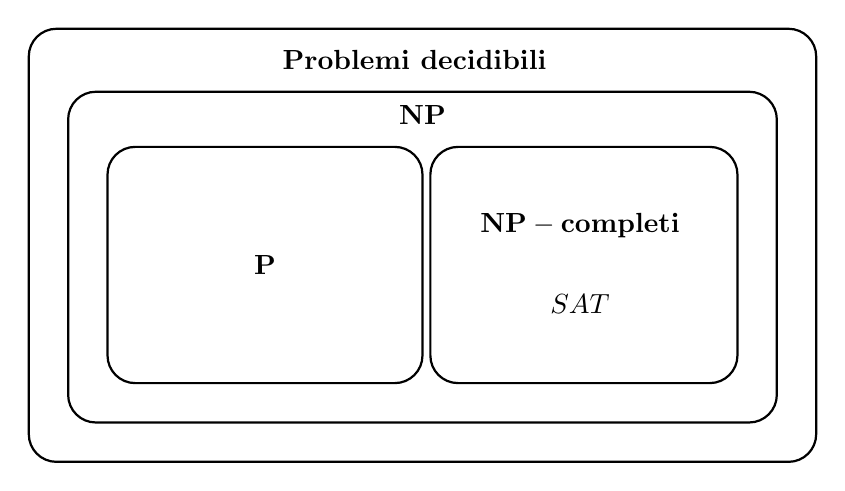
\begin{tikzpicture}[scale=1.0]
		\draw[black,rounded corners=10,thick]
		(0,0) rectangle (10,5.5);
		\draw[black,rounded corners=10,thick]
		(4.9,5.1) node {\bf Problemi decidibili};

		\draw[black,rounded corners=10,thick]
		(0.5, 0.5) rectangle (9.5,4.7);
		\draw[black,rounded corners=10,thick]
		(5,4.4) node {$\mathbf{\mathbf{NP}}$};

		\draw[black,rounded corners=10,thick]
		(1,1) rectangle (5,4);
		\draw[black,rounded corners=10,thick]
		(3,2.5) node {$\mathbf{\mathbf{P}}$};

		\draw[black,rounded corners=10,thick]
		(5.1,1) rectangle (9,4);
		\draw[black,rounded corners=10,thick]
		(7,3) node {\bf $\mathbf{NP-completi}$};
		\draw[black,rounded corners=10,thick]
		(7,2) node {$SAT$};

	\end{tikzpicture}
	\caption{Classi di complessità strutturale.}
	\label{fig:structcomplclass}
\end{figure}

\subsubsection{Riducibilità}
Il concetto di \textbf{riducibilità} (in tempo polinomiale) gioca una parte
fondamentale nella teoria della complessità strutturale: si dice che un problema $\Pi_1$
è polinomialmente riducibile ad un problema $\Pi_2$ se e solo se
$$
	\exists f: 2^* \rightarrow 2^*
$$
tale che:
\begin{itemize}
    \setlength\itemsep{0pt}
	\item $f$ è calcolabile polinomialmente
	\item $\forall x \in I_{\Pi_1}  ~~ f(x) \in I_{\Pi_2}$
	\item $\forall x ~~ Sol_{\Pi_2}(x) = 1 \iff Sol_{\Pi_1}(x) = 1$
\end{itemize}

Questa definizione ha come conseguenza il seguente lemma.
\begin{lemma}\label{lem:poli_red}
	Se $\Pi_2 \in \mathbf{P}$ e $ \Pi_1 \leq_{p} \Pi_2$,
	ossia $\Pi_1$ è riducibile polinomialmente a $\Pi_2$, allora $\Pi_1 \in \mathbf{P}$.
\end{lemma}
La classe dei problemi $\mathbf{NP-completi}$ è quindi definita come
$$
	\mathbf{NP-completi} = \{\Pi \in \mathbf{NP} | \forall \Pi'\in \mathbf{NP} ~~ \Pi' \leq_{p} \Pi\}
$$
\begin{theorem}[di Cook]
	$SAT \in \mathbf{NP-completi}$.
\end{theorem}


%%% Local Variables:
%%% TeX-master: "../main"
%%% End:
